\chapter{Introducción}
En este TFG se ha desarrollado una aplicación web, que pone en contacto profesores y alumnos para dar clases particulares, utilizando tecnologías web de última generación.

Actualmente la web se ha convertido en algo cotidiano entre los mas de 600 millones de usuarios que componen internet, suponiendo un impacto en la economía mundial incalculable. Todo empezó en 1990 cuando Tim Bermers-Lee creó lo que hoy concebimos como web 1.0, una versión inicial de la web que nada tiene que ver con lo que conocemos hoy en día.

Nace como un sistema de hipertexto para compartir información en internet, con la finalidad de publicar documentos. Cuando las empresas empiezan a darse cuenta del potencial de la web, empiezan a incorporar información corporativa con la finalidad de ser más próximos a los clientes y como un canal mas para promocionarse. Pero pronto se dan cuenta de las limitaciones que la web 1.0 contiene:

\begin{itemize}

    \item El contenido publicado no se actualizaba constantemente por lo que podían pasar largos periodos de tiempo sin que esa información se modificase.

    \item Las páginas eran estáticas y no permitían interacción de ningún tipo

    \item La principal desventaja es que eran difícil de manejar y solo podían publicar contenido los más entendidos en el tema o web masters.

\end{itemize}


\begin{figure}[!h]
    \centering
    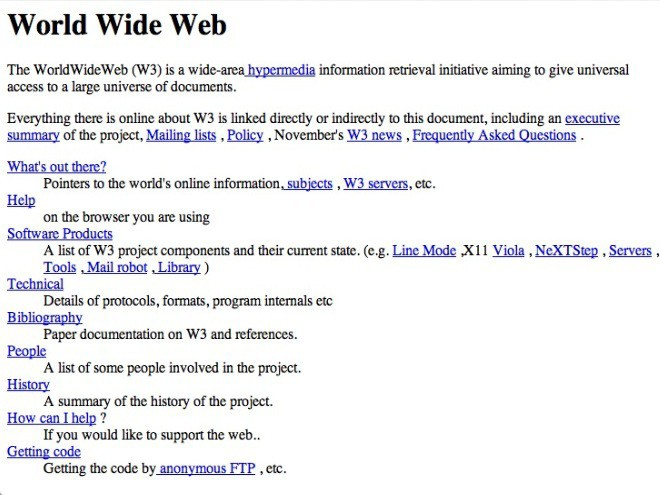
\includegraphics[width=90mm]{img/introduccion/web1.jpg}
    \caption[Ejemplo web 1º generación]{Ejemplo web 1º generación}
\end{figure}

Debido a las limitaciones que ofrece la web 1.0, nace una nueva forma de concebir la web donde se valora las reacciones de los usuarios. Surgen aplicaciones y páginas que utilizan la inteligencia colectiva, consecuencia de ello las páginas pueden ser personalizadas convirtiéndose en una herramienta dinámica que permite el intercambio de información. Es por eso que la información se transforma en comunicación gracias a la interacción y a la incorporación de textos, vídeos, chats… Con esta nueva forma de concebir la web nacen los blogs, las redes sociales, los wikis … Este cambio ha supuesto una gran revolución, puesto que permite devolver la información de los usuarios y poder procesarla con el objetivo de controlar mejor la demanda.


\begin{figure}[!h]
    \centering
    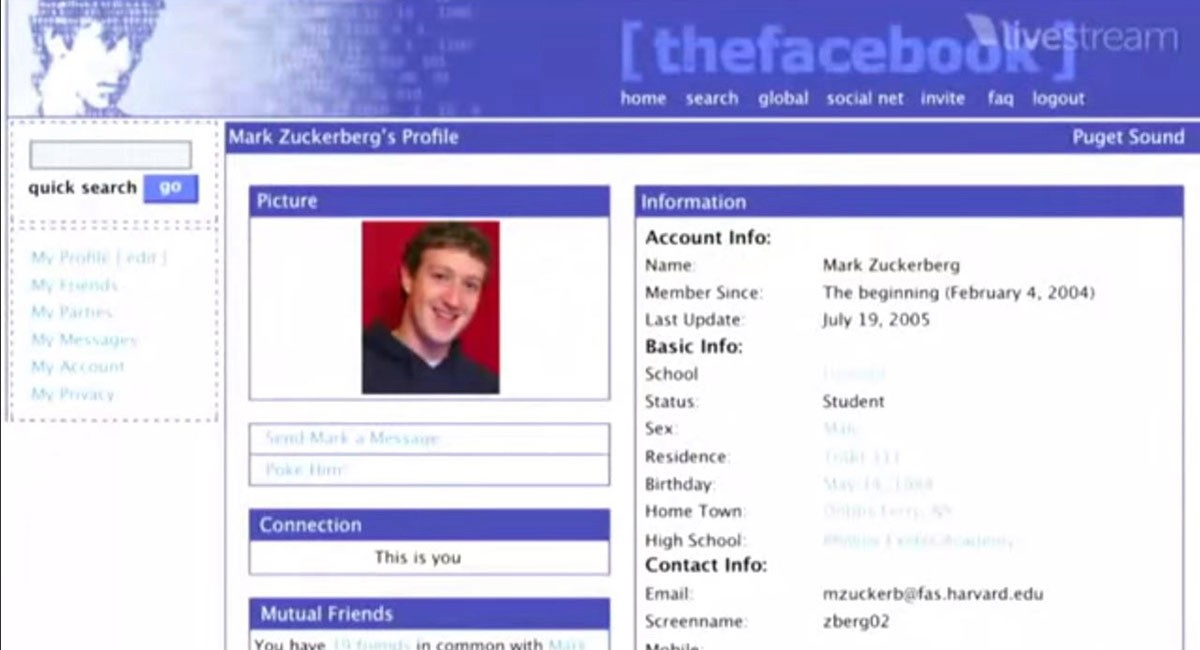
\includegraphics[width=90mm]{img/introduccion/web2.jpeg}
    \caption{Ejemplo web 2º generación}
\end{figure}

La conocida web 3.0 dará paso a otro tipo de web donde pondrá su objetivo en la inteligencia artificial, un método para que los usuarios puedan no solo encontrar la información sino comprenderla. Este control esta en manos de motores informáticos y procesadores de información, que tratan de analizar nuestro perfil y nuestra actividad en red para enviarnos información de nuestro interés.
Es por esto que la web 3.0 es definida por el concepto "personalización", ya que pretende devolver al usuario una información lo más afinada posible, filtrada a sus gustos y preferencias, evitando información que no sea de su interés.

\begin{figure}[!h]
    \centering
    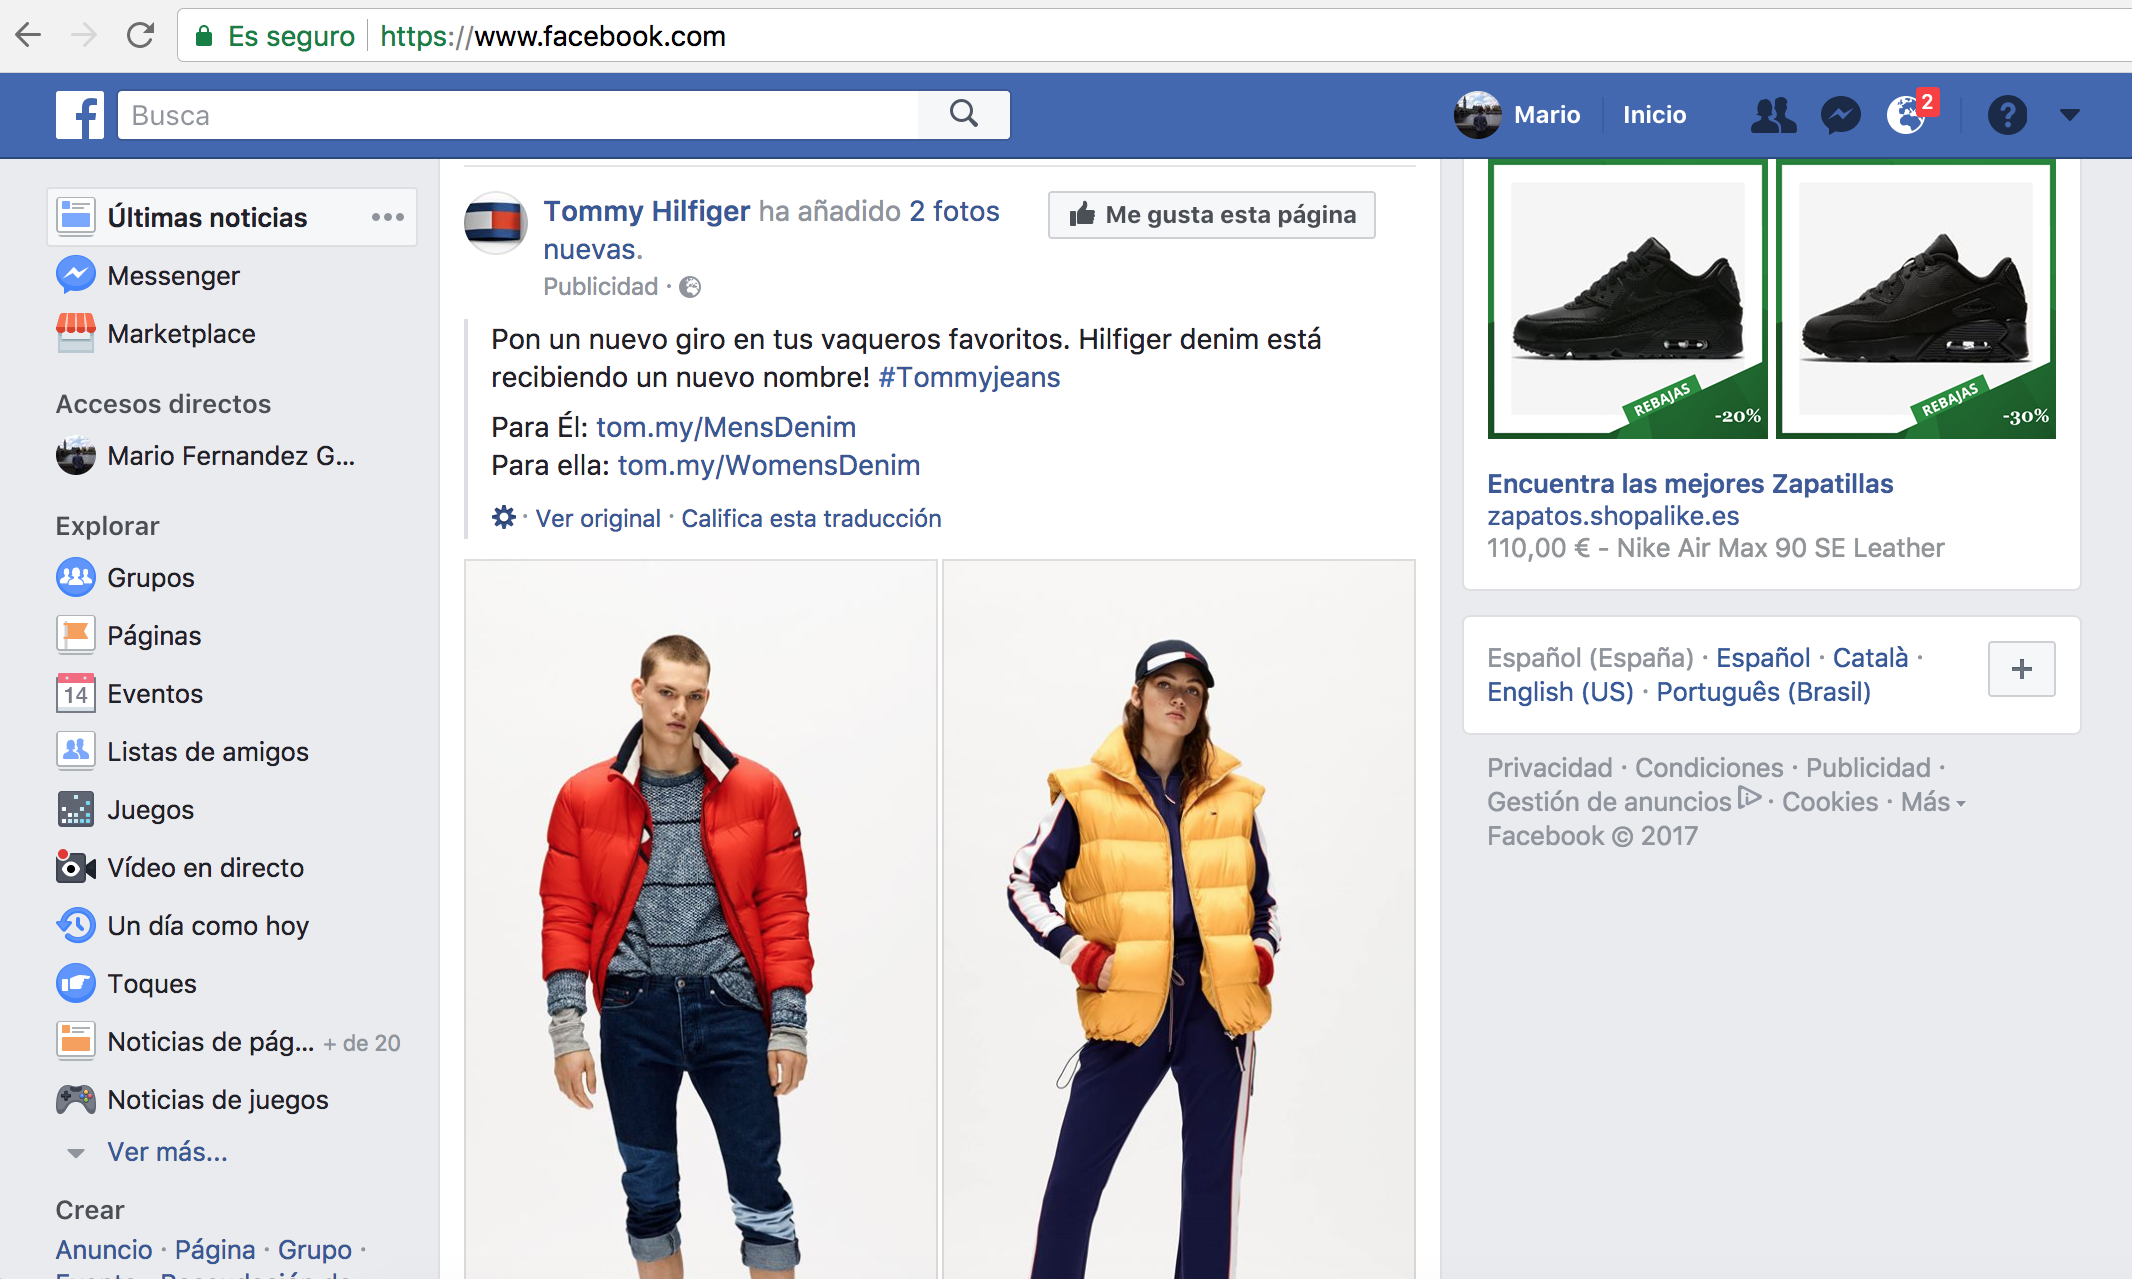
\includegraphics[width=100mm]{img/introduccion/facebook.png}
    \caption{Ejemplo web 3º generación}
\end{figure}

La aplicación de este TFG ha sido desarrollada basándose en modelos de aplicaciones que hoy en día están funcionando, como por ejemplo:

\subsection*{Airbnb}

Es una empresa y una plataforma de software dedicada a la oferta de alojamientos a particulares y turísticos. El nombre es un acrónimo de airbed and breakfast (colchón inflable y desayuno). Airbnb tiene una oferta de unas 2.000.000 propiedades en 192 países y 33.000 ciudades. Desde su creación en noviembre de 2008 hasta junio de 2012 se realizaron 10 millones de reservas.

\begin{figure}[!h]
    \centering
    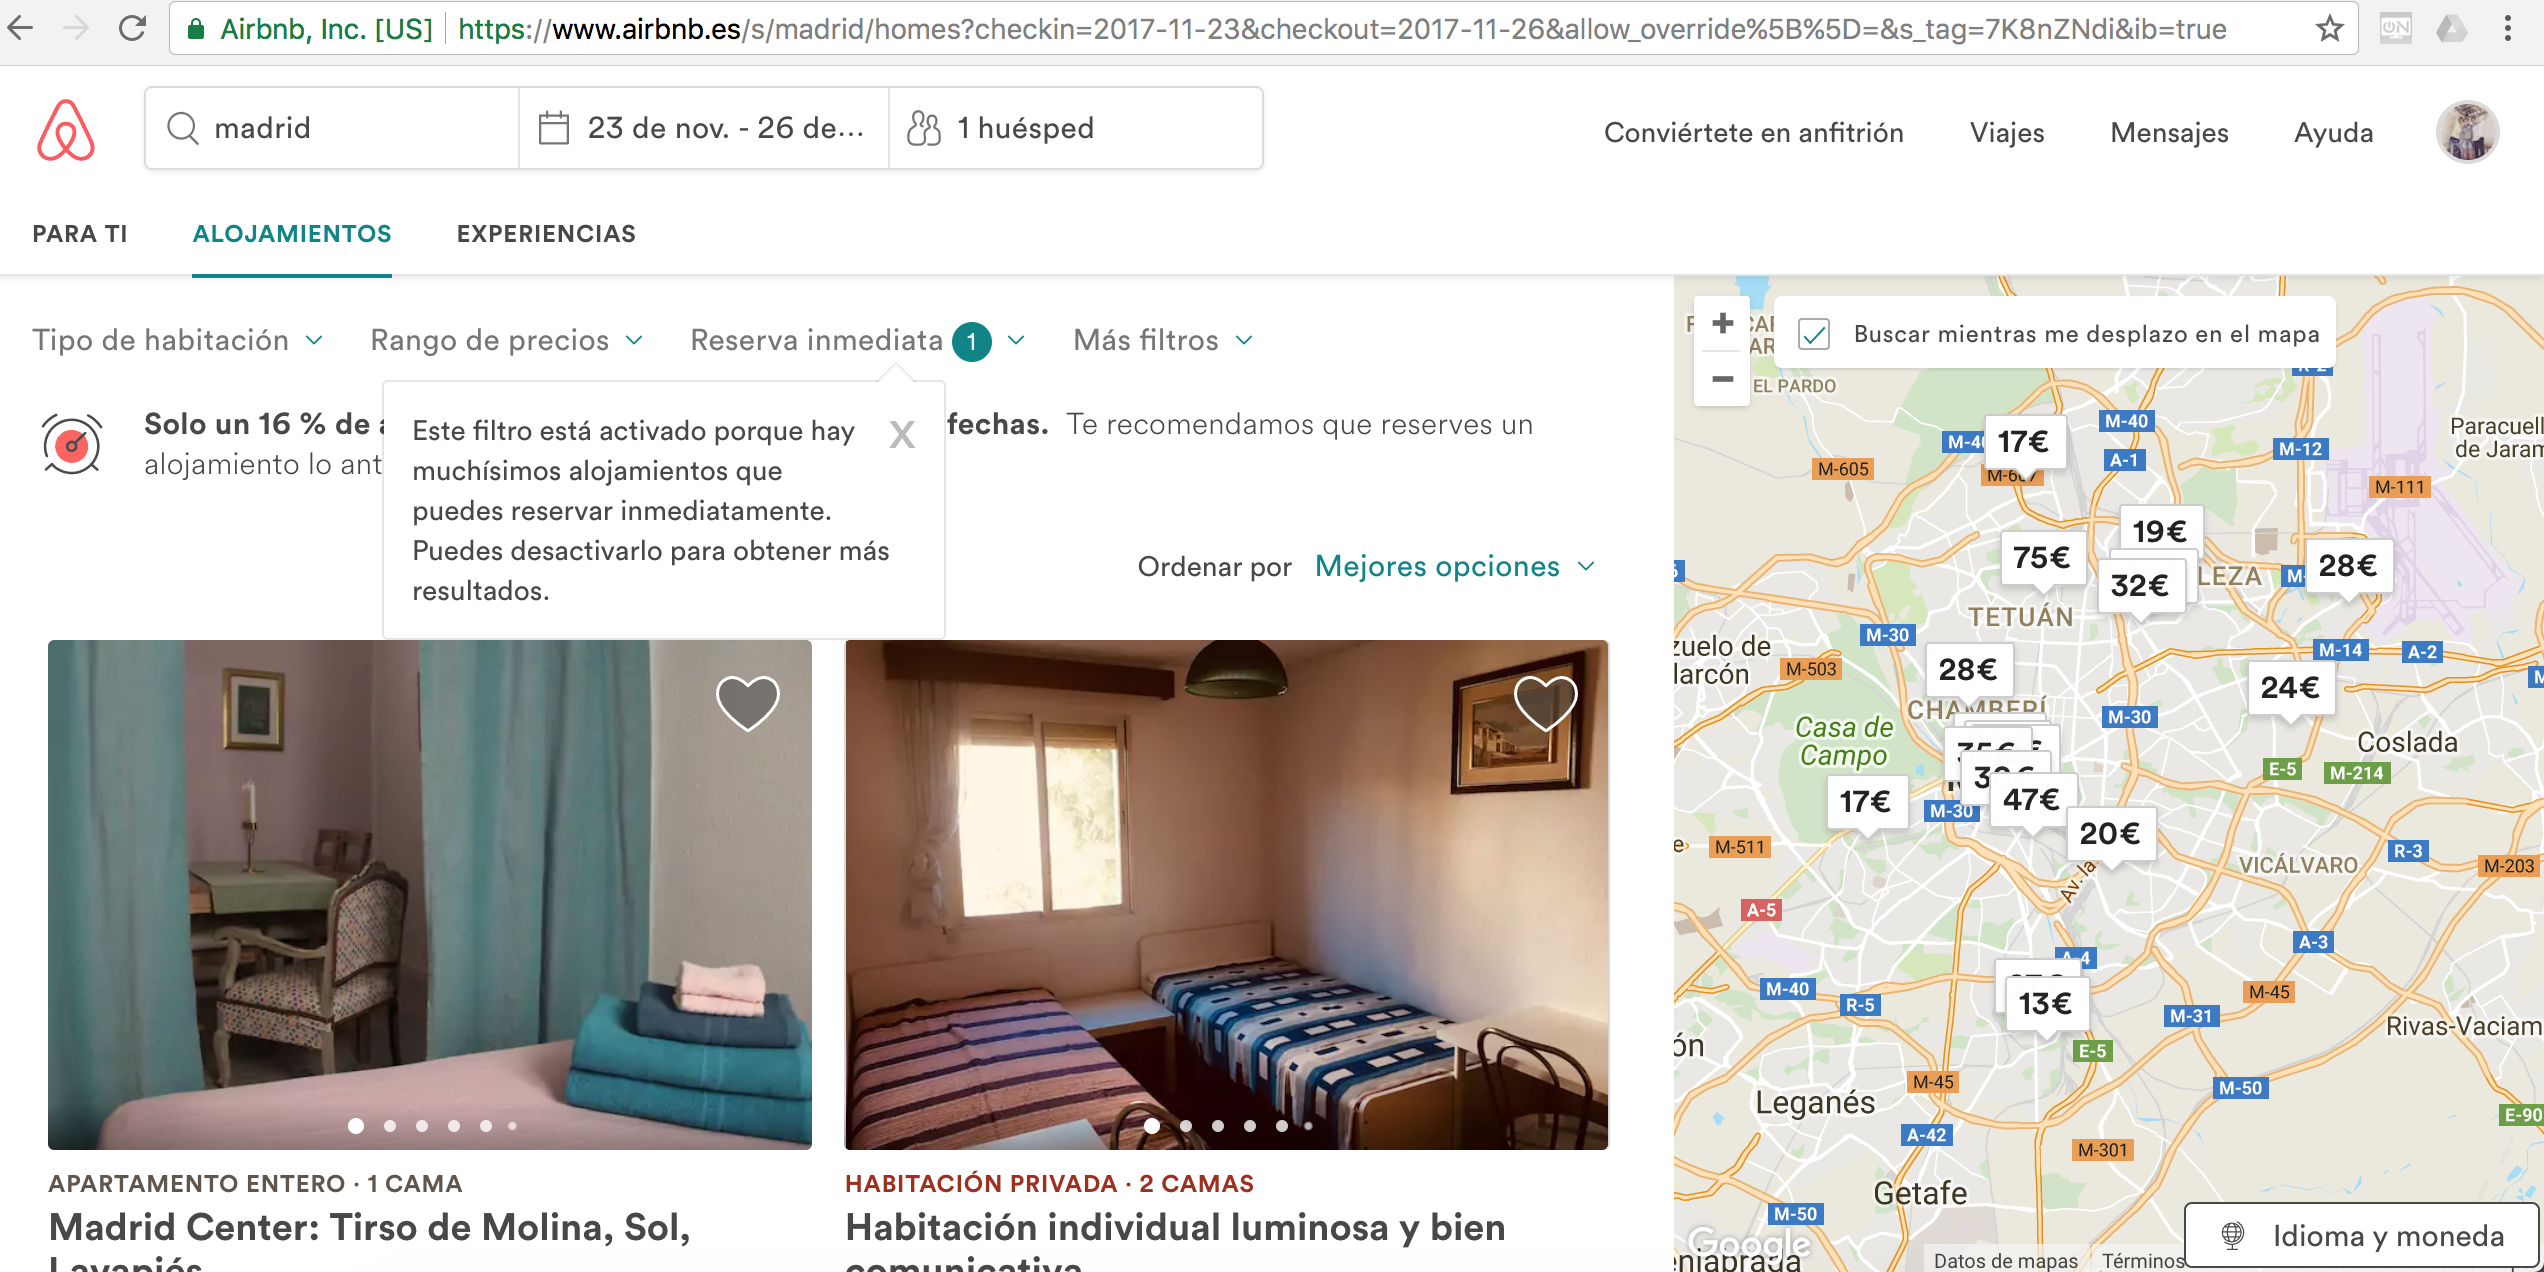
\includegraphics[width=100mm]{img/introduccion/airbnb.png}
    \caption{Aplicación Airbnb}
\end{figure}

\subsection*{Blablacar}

Es un servicio de vehículo compartido que hace posible que las personas que quieren desplazarse al mismo lugar al mismo momento puedan organizarse para viajar juntos. Permite compartir los gastos puntuales del viaje (combustible y peajes) y también evitar la emisión extra de gases de efecto invernadero, al permitir una mayor eficiencia energética en el uso de cada vehículo.

\begin{figure}[!h]
    \centering
    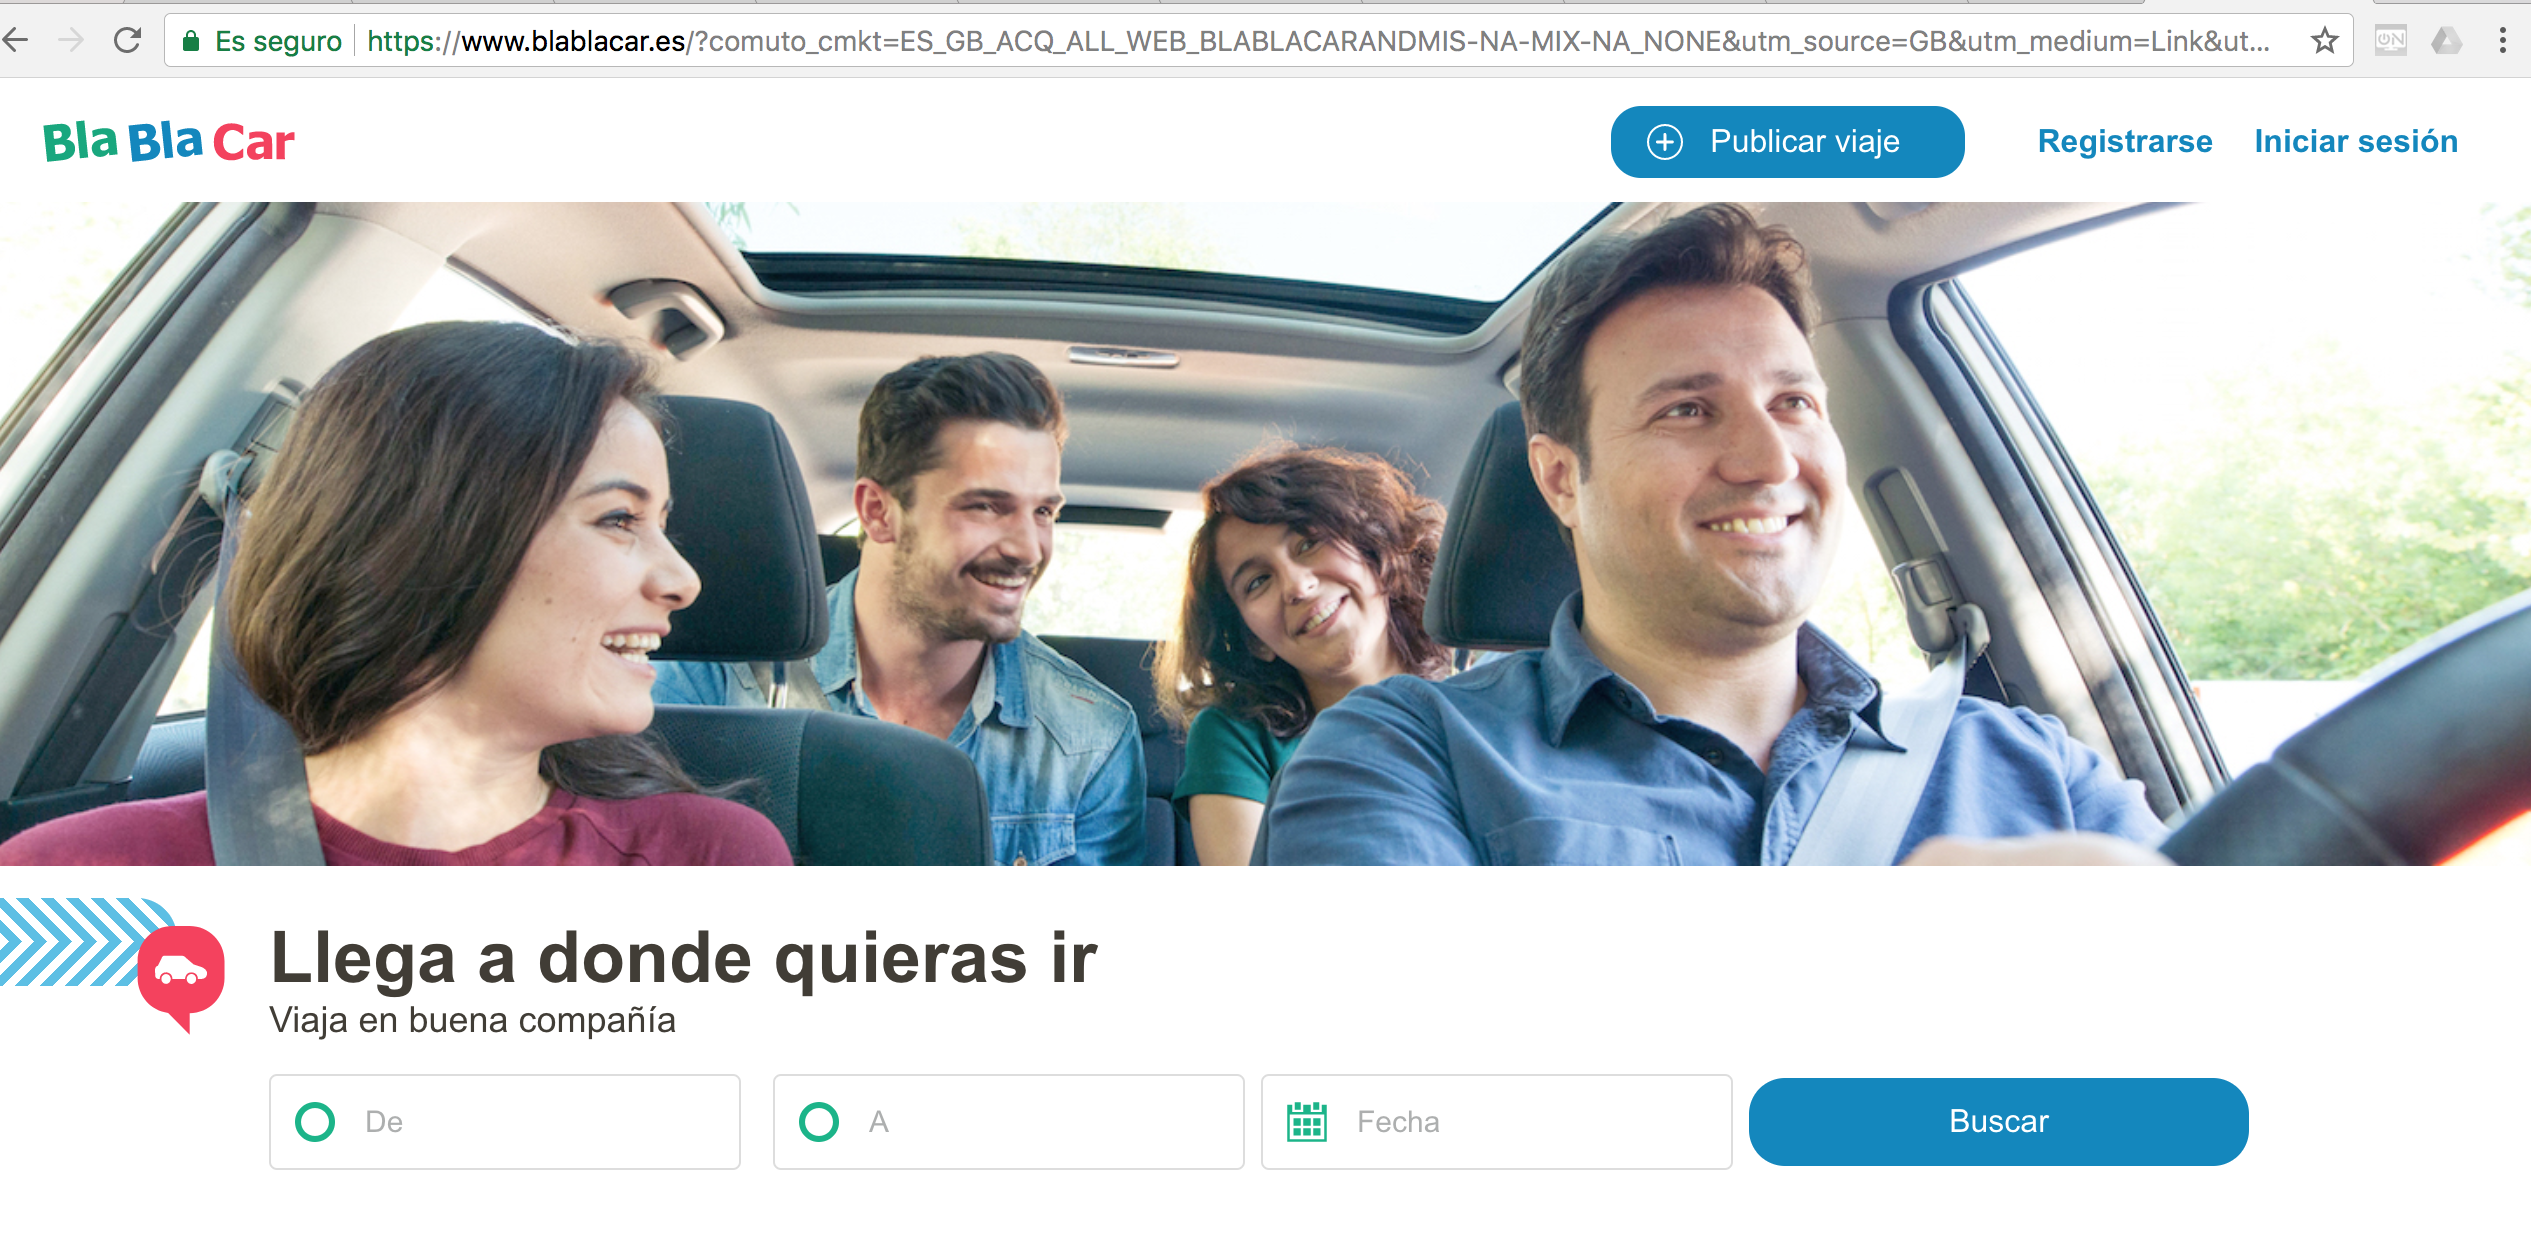
\includegraphics[width=120mm]{img/introduccion/blablacar.png}
    \caption{Aplicación Blablacar}
\end{figure}

\subsection*{Wallapop}

Es una empresa española fundada en 2013, que ofrece un website dedicado a la compra y venta de productos de segunda mano entre usuarios a través de Internet, con un uso centrado en smartphones. Utiliza la geolocalización para que los usuarios puedan comprar y vender en función de su proximidad geográfica

\begin{figure}[!h]
    \centering
    
\includegraphics[width=80mm]{img/introduccion/Wallapop-iPhone.jpg}
    \caption{Aplicación Wallapop}
\end{figure}


\section{Tecnologías web}

Las aplicaciones web como acabamos de comentar han ido evolucionando a lo largo de la historia de internet, pero todas ellas se basan en un modelo cliente-servidor, es decir, para poder lograr la comunicación necesitamos un cliente, normalmente un navegador y un servidor web capaz de atender nuestras solicitudes.

Todas ella se basan en el protocolo HTTP, el cual permite las transferencias de información en la World Wide Web y define la sintaxis y la semántica que utilizan los elementos de software de la arquitectura web (clientes, servidores, proxies) para comunicarse.

\begin{figure}[!h]
    \centering
    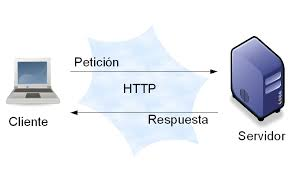
\includegraphics[width=90mm]{img/introduccion/cliente-server.jpeg}
    \caption[Modelo cliente-servidor]{Modelo cliente-servidor}
\end{figure}


\subsection*{HTTP}
HTTP (Hipertext Transfer Protocol) es el protocolo de comunicación que permite la trasferencia de información en la red. Es un protocolo orientado a transacciones y que sigue un esquema petición-respuesta entre un cliente y un servidor.

HTTP define una serie predefinida de métodos de petición(verbos) que pueden utilizarse, teniendo la flexibilidad de ir añadiendo nuevos métodos con sus nuevas funcionalidades.

Entre todos los métodos de petición de HTTP destacamos los siguientes:
\begin{itemize}
    \item \textbf {HEAD:} El método HEAD pide una respuesta idéntica a la de una petición GET, pero sin el cuerpo de la respuesta.
    \item \textbf {GET:} El método GET  solicita una representación de un recurso específico. Las peticiones que usan el método GET sólo deben recuperar datos.
    \item \textbf {POST:} El método POST se utiliza para enviar una entidad a un recurso en específico, causando a menudo un cambio en el estado o efectos secundarios en el servidor.
    \item \textbf {PUT:} El modo PUT reemplaza todas las representaciones actuales del recurso de destino con la carga útil de la petición.
    \item \textbf {DELETE} El método DELETE borra un recurso en específico.
\end{itemize}

HTTP es un protocolo sin estado, es decir, no guarda ninguna información sobre conexiones anteriores. El desarrollo de aplicaciones web necesita frecuentemente mantener estado por lo que se utilizan las cookies, que es información que un servidor puede almacenar en el sistema cliente para simular la noción de la sesión.

\subsection*{API REST}

API REST se define por ser un tipo de arquitectura de desarrollo web que se apoya totalmente en el estándar HTTP.
La arquitectura de un sitio Web tiene tres componentes principales:
\begin{itemize}
    \item \textbf {Un servidor Web:} Distribuye páginas de información formateada a los clientes que las solicitan. Los requerimientos son hechos a través de una conexión de red, y para ello se usa el protocolo HTTP.
    \item \textbf {Una conexión de red}
    \item \textbf {Uno o más clientes:} Una vez que se solicita esta petición mediante el protocolo HTTP y la recibe el servidor Web, éste localiza la página Web en su sistema de archivos y la envía de vuelta al cliente que la solicitó.
\end{itemize}
\begin{figure}[!h]
\centering
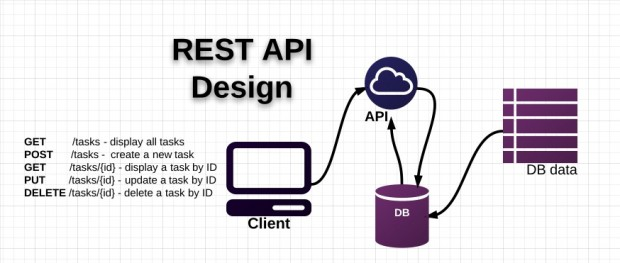
\includegraphics[width=90mm]{img/introduccion/rest-api.jpg}
\caption{api-rest}
\end{figure}

Para comprender el concepto API-REST, primero debemos entender el concepto API. Una API es una interfaz de programación de aplicaciones (del inglés API: Application Programming Interface), que en su conjunto de rutinas provee acceso a funciones de un determinado software.

REST(Transferencia de Estado Representacional) es cualquier interfaz entre sistemas que use HTTP para obtener datos o generar operaciones sobre esos datos en todos los formatos posibles, como XML y JSON. Es una alternativa en auge a otros protocolos estándar de intercambio de datos como SOAP (Simple Object Access Protocol), que disponen de una gran capacidad pero también mucha complejidad. A veces es preferible una solución más sencilla de manipulación de datos como REST.

Las reglas que definen una API-REST son las siguientes:
\begin{itemize}
    \item \textbf {Interfaz uniforme: } para la transferencia de datos en un sistema REST, este aplica acciones concretas (POST, GET, PUT y DELETE) sobre los recursos, siempre y cuando estén identificados con una URI.
    \item \textbf {Peticiones sin estado} cada petición HTTP contiene toda la información necesaria para ejecutarla, lo que permite que ni cliente ni servidor necesiten recordar ningún estado previo para satisfacerla.
    \item \textbf {Cacheable} existe la posibilidad de definir algunas respuestas a peticiones HTTP concretas como cacheables, con el objetivo de que el cliente pueda ejecutar en un futuro la misma respuesta para peticiones idénticas.
    \item \textbf {Separación de cliente y servidor}
    \item \textbf {Sistema de Capas} arquitectura jerárquica entre los componentes. Cada una de estas capas lleva a cabo una funcionalidad dentro del sistema REST.
\end{itemize}

La arquitectura API-REST donde las comunicaciones son más ligeras entre productor y consumidor, mantenibles y escalables, hacen de REST un estilo de construcción popular para APIs basadas en la nube, como las proporcionadas por Amazon, Microsoft y Google.

El estilo REST hace énfasis en que las interacciones entre los clientes y los servicios se mejoran al tener un número limitado de operaciones (verbos). La flexibilidad se obtiene asignando recursos a sus propios identificadores de recursos universales únicos (URI). Debido a que cada verbo tiene un significado específico (GET, POST, PUT y DELETE), evitando la ambigüedad.
\begin{itemize}
    \item \textbf {GET} Se usa GET para obtener un recurso
    \item \textbf {POST}Se usa POST para crear un recurso en el servidor
    \item \textbf {PUT} Se usa PUT para cambiar el estado de un recurso o actualizarlo
    \item \textbf {DELETE} Se usa DELETE para eliminar un recurso
\end{itemize}

\subsection*{Paradigma MVC}
MVC es un patrón que separa completamente los datos, la lógica de negocio y la interfaz de usuario de una aplicación. Esto ayuda a la reutilización de código y su mantenimiento.
Veámos en qué se centra cada parte:
\begin{itemize}
\item \textbf {El modelo} es la información que maneja nuestra aplicación y su estructura.
\item \textbf {En el controlador} es donde reside la lógica de negocio y, por tanto, será el encargado de procesar los datos y hacer operaciones con ellos. Por otro lado, también es el puente de comunicación entre los datos y las vistas.
\item \textbf {Las vistas} suelen ser puras representaciones de los datos ofrecidos por el controlador.
\end{itemize}
\begin{figure}[!h]
    \centering
    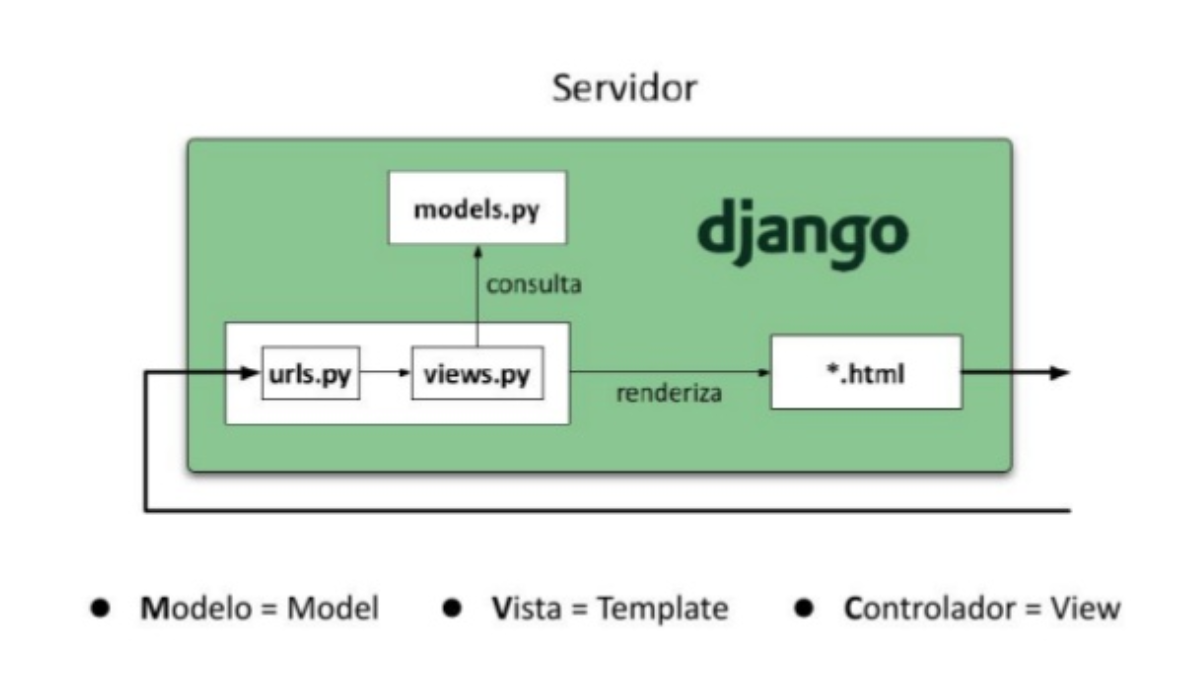
\includegraphics[width=90mm]{img/introduccion/mvc.png}
    \caption{Diagrama de MVC}
\end{figure}

\section{Tecnologías del Cliente}

El Front-end se desarrolla normalmente en HTML, CSS o Javascript, lo cual implica que los programadores se especialicen en estos tres lenguajes. Además de que el código sea correcto, la web debe tener un diseño atractivo y funcional, que permita que la experiencia del usuario sea lo suficientemente cómoda, intuitiva y agradable para que continúe navegando.

\subsection{HTML 5}
\begin{figure}[!h]
    \centering
    
\includegraphics[width=40mm]{img/introduccion/html5.png}
    \caption{HTML5 Icono}
\end{figure}
HTML5 es la quinta versión del lenguaje básico de la Worl Wide Web, publicado en Octubre de 2014. Al no ser reconocido en viejas versiones de navegadores por sus nuevas etiquetas, se recomienda al usuario común actualizar su navegador a las versión mas reciente, para poder disfrutar de todo el potencial que provee HTML5.

HTML5 incluye significativas novedades en diversos áreas, ya que no incorpora solo nuevas etiquetas o elimina otras, sino que mejora áreas que estaban fuera del alcance del lenguaje:

\begin{itemize}
    \item \textbf{Responsive: } Permite desarrollar aplicaciones que se adaptan fácilmente a distintas resoluciones, tamaños de pantallas, relaciones de aspectos y orientaciones.
    \item \textbf{Geolocalización: }Permite localizar gráficamente las páginas web por medio de una API de geolocalización.
    \item \textbf{Canvas: } Nuevo componente que permitirá dibujar en la página todo tipo de formas, que podrán estar animadas y responder a interacciones del usuario por medio de las funciones de un API.
    \item \textbf{WebSockets } tecnología que proporciona un canal de comunicación bidireccional y full-duplex sobre un único socket TCP.
    \item \textbf{Aplicaciones web Offline } API que permite el trabajo con aplicaciones web, que se podrán desarrollar para que funcione también en local y sin estar conectados a internet.
\end{itemize}
\subsection{ECMAScript 6}
\begin{figure}[!h]
    \centering
    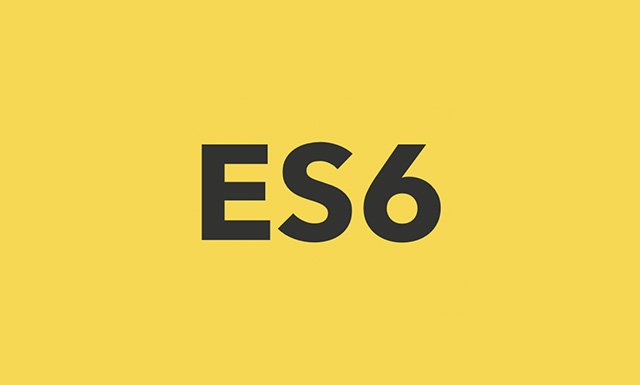
\includegraphics[width=40mm]{img/introduccion/ecma6.jpg}
    \caption{EcmaScript 6 Icono}
\end{figure}
ECMAScript es una especificación estándar de un lenguaje desarrollado por Brendan Eich. Inicialmente se llamaba Mocha, luego LiveScript, y finalmente Javascript. Debido al gran éxito de Javascript como lenguaje de scripting del lado del cliente para paginas web, Microsoft desarrollo un dialecto compatible del lenguaje llamado JScript, para evitar problemas legales con la marca.
La primera versión de JavaScript, ECMAScript 1, se lanzó en Junio de 1997, y desde entonces han existido las versiones 2, 3 y 5, que es la más usada actualmente (la 4 se abandonó). Sobre la versión de ECMAScript 6, podemos decir que desde 2015 ya es un estándar cerrado, tratándose de una evolución del lenguaje JavaScript para dotarlo de características avanzadas que se echaban mucho en falta y que sí estaban disponibles en otros lenguajes populares, como por ejemplo:
\begin{enumerate}
    \item \textbf{Mejoras de sintaxis: } parámetros por defecto, variables let, plantillas...
    \item \textbf{Módulos para organización de código }
    \item \textbf{Verdaderas clases para programación orientada a objetos  }
    \item \textbf{Promesas:  }para programación asíncrona.
    \item \textbf{Mejoras en programación funcional: } expresiones lamda, iteradores, generadores...
\end{enumerate}
Una cuestión muy importante es que ECMAScript 6 es totalmente compatible hacia atrás con versiones anteriores, por lo que no tenemos que preocuparnos por nuestro código actual, el cual funcionará perfectamente en motores de JavaScript que usen la próxima versión.
Centrando el foco en el lenguaje de programación JavaScript, aparecen multitud de framework que facilitan su programación como son Angular2+, Vuejs y React entre otros.
\subsection{CSS3}
\begin{figure}[!h]
    \centering
    
\includegraphics[width=40mm]{img/introduccion/css.jpg}
    \caption{CSS3 Icono}
\end{figure}
CSS o Cascading Style Sheet (Hoja de estilos en cascada) es el lenguaje de diseño de la web.
Su estandarizacion y especificación corre por parte del W3C, que lo incluyo a partir de la versión 4 de HTML.
Gracias a este lenguaje, podremos indicar donde se colocan los elementos, su color, apariencia, etc.
Al tratarse de estilos en cascada, los estilos que definamos en un elemento que contenga a otros, éstos podrán propagarse hacia abajo. Por ejemplo: Si cambiamos el tamaño de fuente al elemento <body>(Padre de todo el documento), todos los párrafos y links de la página tendrán ese tamaño de fuente a menos que indiquemos lo contrario.
En esta última vesión se han incluido grandes mejoras, podemos hacer uso de transformaciones 2D y 3D así como animaciones aceleradas por GPU, lo que hace que sean mucho más suaves y vistosas que programándolas como hasta ahora, en JavaScript.
\subsection{DOM}
Document Object Model o DOM ('Modelo de Objetos del Documento' o 'Modelo en Objetos para la Representación de Documentos') es esencialmente una interfaz de plataforma que proporciona un conjunto estándar de objetos para representar documentos HTML, XHTML y XML un modelo estándar sobre cómo pueden combinarse dichos objetos, y una interfaz estándar para acceder a ellos y manipularlos. A través del DOM, los programas pueden acceder y modificar el contenido, estructura y estilo de los documentos HTML y XML, que es para lo que se diseñó principalmente.

El DOM permite el acceso dinámico a través de la programación para acceder, añadir y cambiar dinámicamente contenido estructurado en documentos con lenguajes como ECMAScript (JavaScript).
\begin{figure}[!h]
    \centering
    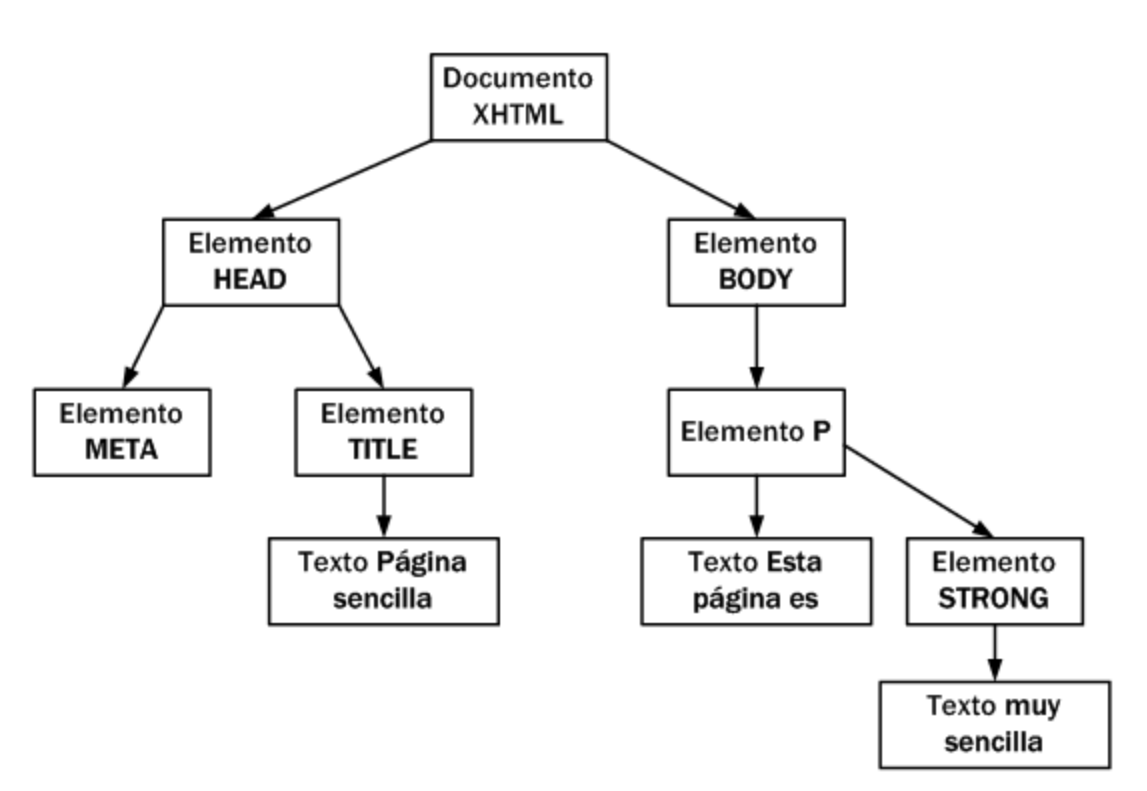
\includegraphics[width=90mm]{img/introduccion/arbol_dom.png}
    \caption{Arbol DOM}
\end{figure}

\subsection{Frameworks}
Un Framework en desarrollo es un conjunto estandarizado de conceptos, prácticas y criterios para enfocar un tipo de problemática particular que sirve como referencia, para enfrentar y resolver nuevos problemas de índole similar.

A continuación se van a describir los principales frameworks de JavaScript para el lado del cliente que existen en la actualidad.
\begin{itemize}
    \item \textbf{Angular: } es el framework estrella hoy en día en demanda de ofertas de trabajo y en comunidad detrás de él.
    La gran crítica de los desarrolladores sobre Angular es su gran curva de aprendizaje, ya que empezar con Angular implica tener unos amplios conocimientos de diferentes tecnologías.
    \item \textbf{React: }es la segunda gran apuesta en el desarrollo de aplicaciones del lado de cliente. Ha sido creado por Facebook para el desarrollo de interfaces de usuario en aplicaciones Web. Constantemente se compara React con Angular pero sus objetivos son diferentes: React no es un framework sino una biblioteca que se centra en crear interfaces de usuario, a diferencia de Angular, que trata de abarcar mucho más.
    \item \textbf{Vue.js: } El tercer framework en esta lista es el proyecto de código abierto denominado Vue.js, el cual ha tenido una gran popularidad en los últimos tiempos con la aparición de la versión 2.0 en 2016. Este framework trata de tomar lo mejor de cualquier framework e implementarlo, de hecho, en amplias comparativas entre diferentes frameworks ha conseguido unos resultados extraordinarios en velocidad y ligereza de peso
\end{itemize}
\section{Tecnología del Servidor}
\begin{figure}[!h]
    \centering
    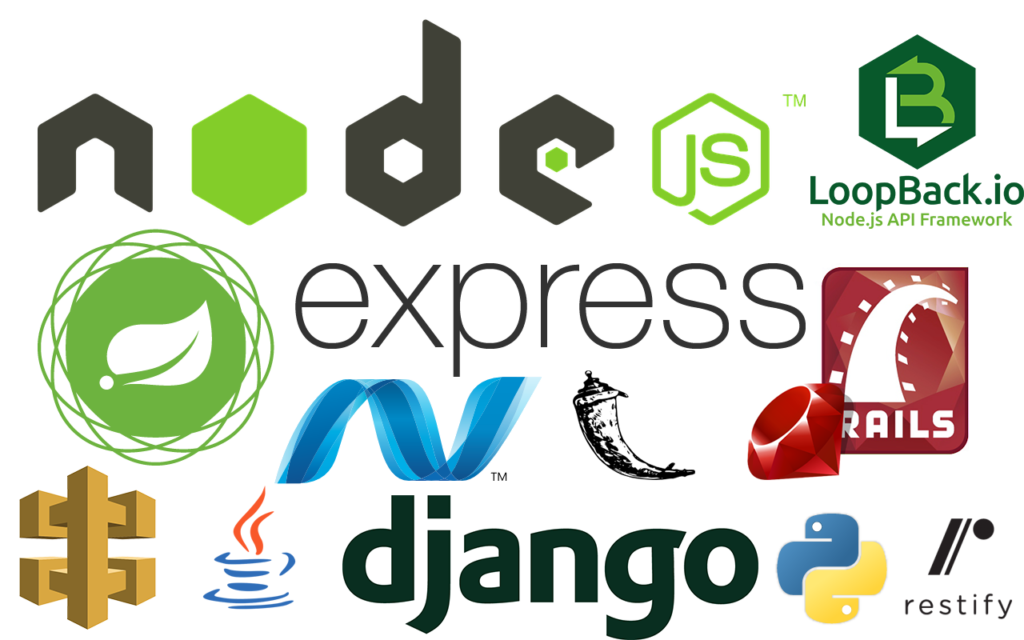
\includegraphics[width=60mm]{img/introduccion/frameworks-backend.png}
    \caption{CSS3 Icono}
\end{figure}
Un servidor web o servidor HTTP es un programa informático que procesa una aplicación del lado del servidor, realizando conexiones bidireccionales o unidireccionales y síncronas o asíncronas con el cliente y generando o cediendo una respuesta en cualquier lenguaje o Aplicación del lado del cliente. El código recibido por el cliente es renderizado por un navegador web.

La principal razón para usar servicios Web es que se pueden utilizar con HTTP sobre Transmission Control Protocol (TCP) en el puerto de red 80. Dado que las organizaciones protegen sus redes mediante firewalls (que filtran y bloquean gran parte del tráfico de Internet), cierran casi todos los puertos TCP salvo el 80, que es, precisamente, el que usan los navegadores web. Los servicios Web utilizan este puerto, por la simple razón de que no resultan bloqueados. Es importante señalar que los servicios web se pueden utilizar sobre cualquier protocolo, sin embargo, TCP es el más común.

\subsection*{Frameworks}
Los frameworks de lado servidor nos hacen más fácil escribir, mantener y escalar aplicaciones web. Los principales son:
\begin{itemize}
    \item \textbf{Express: } es un framework web veloz, no dogmático, flexible y minimalista para Node.js. Proporciona un conjunto de características para aplicaciones web y móviles. Express es extremadamente popular, en parte porque facilita la migración de programadores web de JavaScript de lado cliente a desarrollo de lado servidor, y en parte porque es eficiente con los recursos
    \item \textbf{Django: } es un Framework Web Python de alto nivel que promueve el desarrollo rápido y limpio y el diseño pragmático. Es también veloz, seguro y muy escalable. Al estar basado en Python, el código de Django es fácil de leer y de mantener.
    \item \textbf{Ruby on rails: } es un framework web escrito para el lenguaje de programación Ruby. Rails sigue una filosofía de diseño muy similar a Django. Como Django proporciona mecanismos estándard para el enrutado de URLs, acceso a datos de bases, generación de plantillas y formateo de datos como JSON o XML.
\end{itemize}

\section{Computación en la nube}
Otra de las tecnologías usadas en este TFG es la computación en la nube. Esta computación en la nube es un paradigma que permite ofrecer servicios de computación a través de internet. Cuando los proveedores utilizan la palabra cloud, se refieren a la posibilidad de configurar y redimensionar los recursos que se usan de forma rápida y sencilla, o manualmente vía web o usando APIs REST.

Este tipo de servicios son tan dinámicos que se cobran por horas o minutos dependiendo de la plataforma de computación en la nube. Además los recursos de computación en la nube suelen estar virtualizados, aunque en algunas ocasiones pueden ser maquinas físicas.
\begin{figure}[!h]
    \centering
    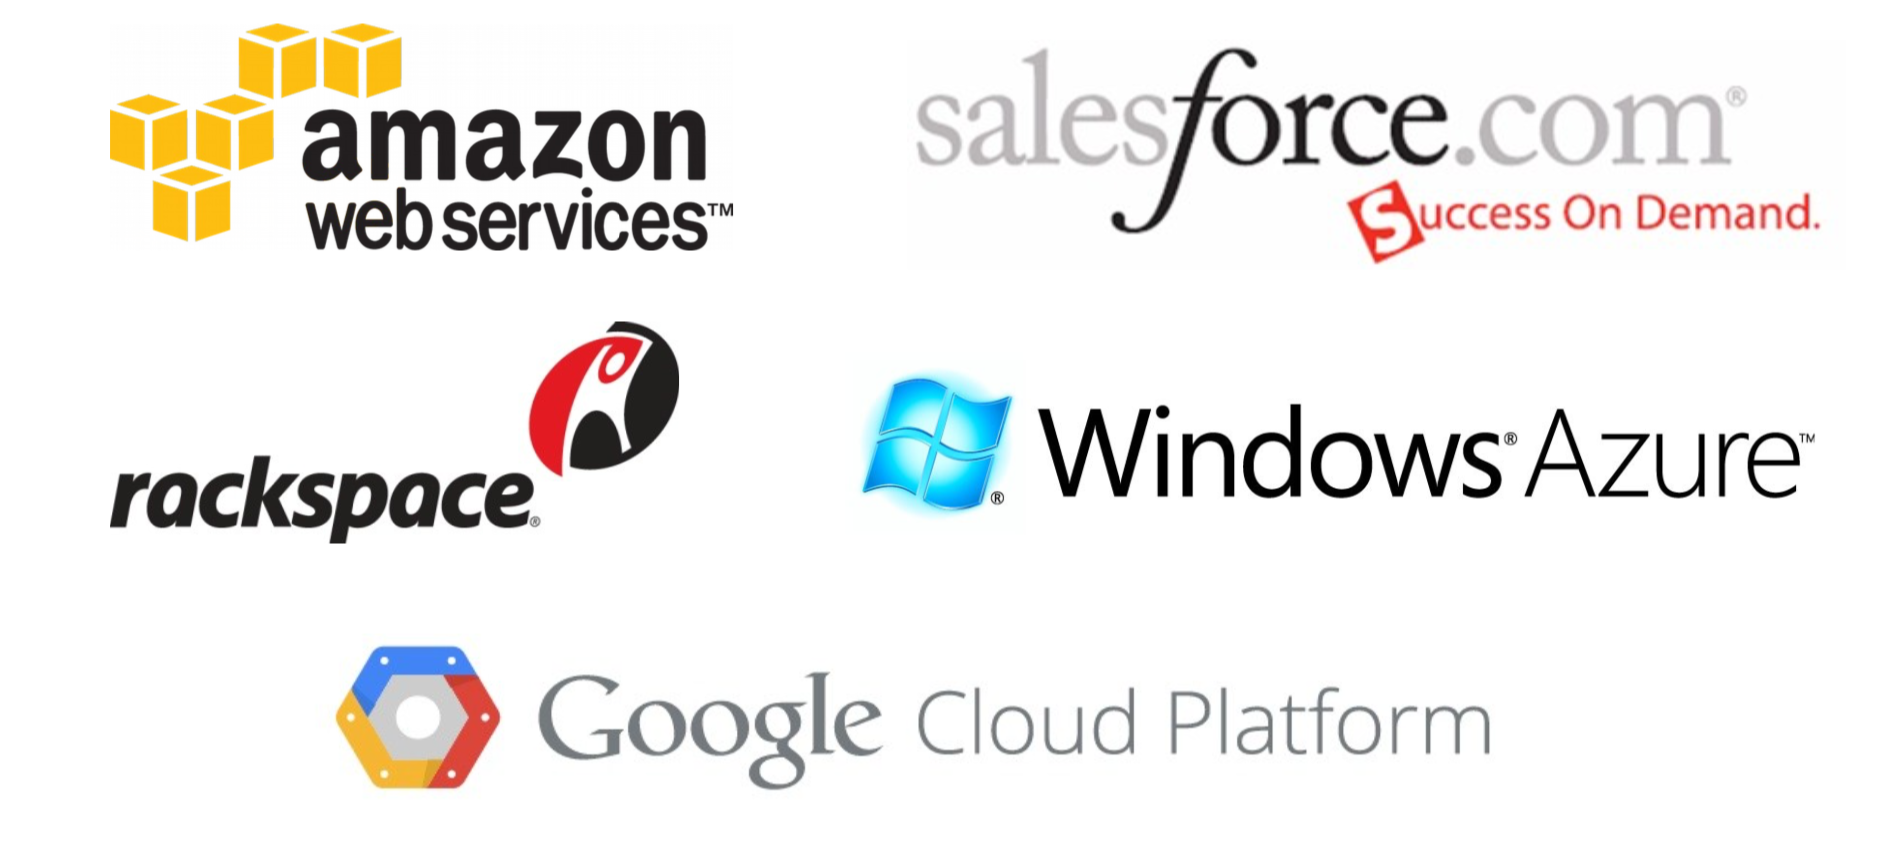
\includegraphics[width=100mm]{img/despliegue/proveedores.png}
    \caption{Proveedores más conocidos de computación en la nube}
\end{figure}

Los proveedores de la computación en la nube ofrecen diferentes tipos de servicios, tanto de bajo nivel como de alto nivel.

\begin{enumerate}
     \item \textbf{Servidores virtuales (Instancias)}
    \item \textbf{Gestión del sistema operativo que tendrán los servidores (Imagen)}
    \item \textbf{Sistemas de copia de seguridad de los servidores completos }
    \item \textbf{Balanceadores de carga entre servidores}
    \item \textbf{Bases de datos administradas }
    \item \textbf{Servicios de gestión de logs, monitorización y alarmas}
    \item \textbf{Plataforma auto-escalable para ejecución de aplicaciones}
\end{enumerate}

Los servicios ofrecidos por los porveedores pueden ser de diferentes tipos de abstraccion:

\begin{enumerate}
     \item \textbf{Infraestructura como servicio (IaaS): } IaaS proporciona acceso a recursos informáticos situados en un entorno virtualizado, la 'nube' (cloud), a través de una conexión pública. En el caso de IaaS, los recursos informáticos ofrecidos consisten en infraestructura de procesamiento. La definición de IaaS abarca aspectos como el espacio en servidores virtuales, conexiones de red, ancho de banda, direcciones IP y balanceadores de carga.
    \item \textbf{Plataforma como Servicio (PaaS): }El modelo PaaS permite a los usuarios crear aplicaciones de software utilizando herramientas suministradas por el proveedor. Los servicios PaaS pueden consistir en funcionalidades preconfiguradas a las que los clientes puedan suscribirse, eligiendo las funciones que deseen incluir para resolver sus necesidades y descartando aquellas que no necesiten.
    \item \textbf{Software como Servicio (SaaS): } El modelo SaaS se conoce también a veces como "software bajo demanda", y la forma de utilizarlo se parece más a alquilar el software que a comprarlo. Con las aplicaciones tradicionales el software se compra al principio como un paquete, y una vez adquirido se instala en el ordenador del usuario. La licencia del software puede también establecer limitaciones en cuanto al número de usuarios y/o dispositivos en los cuales puede instalarse.

\end{enumerate}

Cada vez son más las empresas que deciden utilizar la computación en la nube ya que desde 2006, , Amazon Web Services proporciona servicios de infraestructura de TI para empresas en forma de servicios web.
Uno de los principales beneficios de la computación en la nube es la oportunidad de reemplazar importantes gastos de infraestructura con costes reducidos que se escalan dependiendo de la dimensión de su negocio.
Gracias a la nube, las empresas ya no tienen que planificar ni adquirir servidores y otra infraestructura de TI con semanas o meses de antelación. Pueden disponer en cuestión de minutos de cientos o de miles de servidores y ofrecer resultados más rápidamente.

\section{Antecedentes}
EL TFG centra su desarrollo en el campo de las tecnologías Web y como a través de ella permiten generar diversas aplicaciones con las que el usuario puedan interactuar. A continuación, se presentan varios ejemplos de TFGs dentro del Laboratorio de Robótica de la URJC que emplean estas tecnologías y han sido el punto de partida de este TFG.

\subsection*{Suveillance 5.1}
Edgar barrero desarrollo en Ruby sobre Rails Suveillance 5.1 \cite{TFGsurveillance5.1}\cite{surveillance5.1}, una aplicación web que ofrece un flujo de vídeo desde una cámara web, un flujo de imagen de profundidad procedente de un sector Kinect y su representación en 3D, además de un sensor de humedad y un actuador.


\begin{figure}[!h]
    \centering
    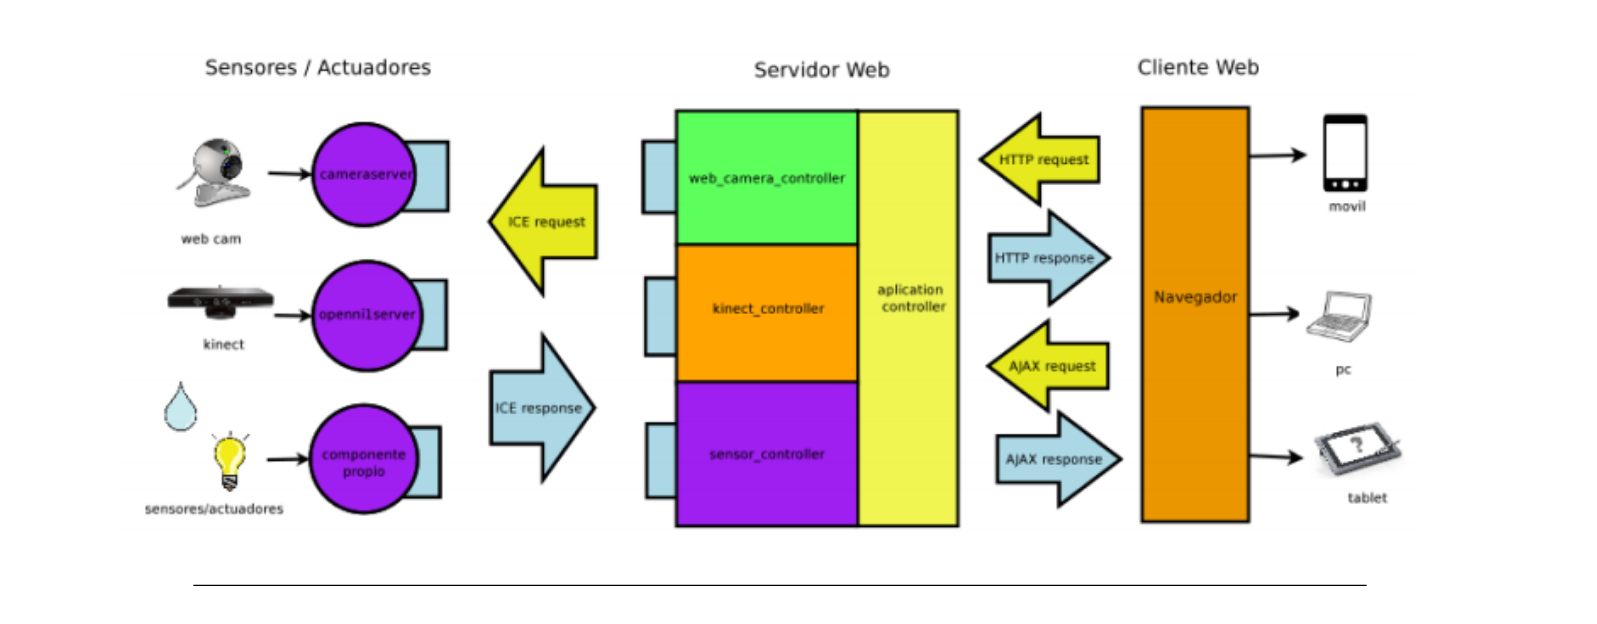
\includegraphics[width=150mm]{img/introduccion/edgar.png}
    \caption{TFG Edgar Barrero}
\end{figure}

\subsection*{Prácticas docentes de desarrollo web}
Este TFG\cite{TFGPracticasDesarrolloWeb}\cite{PracticasDesarrolloWeb} fué realizado por Walter Cuenca, con el objetivo de servir como apoyo en las prácticas de la asignatura de LTAW del grado de ingeniería de sistemas audiovisuales y multimedia. Consta de cuatro prácticas que utilizan diferentes tecnologías Web, herramientas y bibliotecas muy acentuadas en este campo. Algunas de las tecnologías empleadas son Javascript en el cliente, NodeJS y Django en el servidor, Base de datos como MySQL y por último Web-Socket y WebRTC como tecnologías de comunicación fluida.
\url{https://github.com/RoboticsURJC-students/2015-TFG-Walter-Cuenca}


\subsection*{JdeRobotWebClients (URJC)}
JdeRobotWebClients \cite{TFGJdeRobotWebClients}\cite{JdeRobotWebClients}fue desarrollado por Aitor Martınez Fernandez como trabajo fin de grado. La aplicación Web consiste en crear seis versiones web de herramientas utilizadas por JdeRobot (CameraViewJS, RGBDViewerJS, KobukiViewerJS, .....) que estaban programadas en C++ o Python con su propio interfaz gráfico provocando que sean ejecutables solo en Linux.
Estas nuevas versiones son multiplataforma (Linux, Android, IOS, Windows) y accesibles desde un navegador web como interfaz gráfico permitiendo acceder a los sensores y actuadores sin un servidor intermedio.

\begin{figure}[!h]
    \centering
    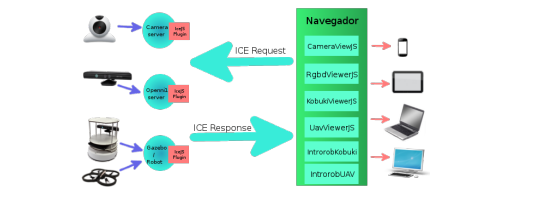
\includegraphics[width=150mm]{img/introduccion/jdro.png}
    \caption{TFG Aitor Martinez Fernandez}
\end{figure}
